%!TEX root = ./Body.tex

\chapter{Features} % (fold)
\label{cha:Features}

\section{Strukturierung} % (fold)
\label{sec:Strukturierung}
Feature Extraktion. See figure ~\ref{fig:feature_extraction}.\\

Generierung von Feature-Vektoren für alle Referenz-Fahrt-Paare.\\

Normalisierung
\begin{itemize}
\item Numerische Stabilität
\item Ausreißer vermeiden
\end{itemize}

Zusammenfassen in Feature-Liste
\begin{itemize}
\item Leichte Verarbeitung
\end{itemize}

\begin{figure}[htbp]
\begin{center}
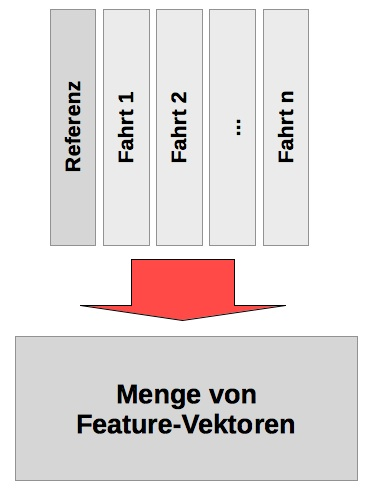
\includegraphics[width=0.3\textwidth]{feature_extraction}
\caption{Feature Extraction}
\label{fig:feature_extraction}
\end{center}
\end{figure}

Überblick über die Features. See figure ~\ref{fig:feature_overview}.\\

\begin{figure}[htbp]
\begin{center}
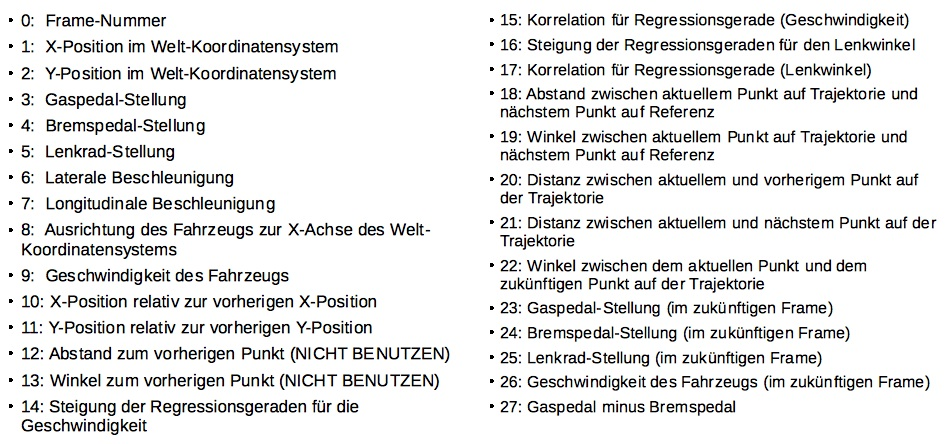
\includegraphics[width=1\textwidth]{feature_overview}
\caption{Feature Overview}
\label{fig:feature_overview}
\end{center}
\end{figure}
% section Strukturierung (end)


\section{Berechnung der benutzten Features} % (fold)
\label{sec:Berechnung_der_benutzten_Features}
Vektoren. See figure ~\ref{fig:feature_vektoren}.\\

\begin{figure}[htbp]
\begin{center}
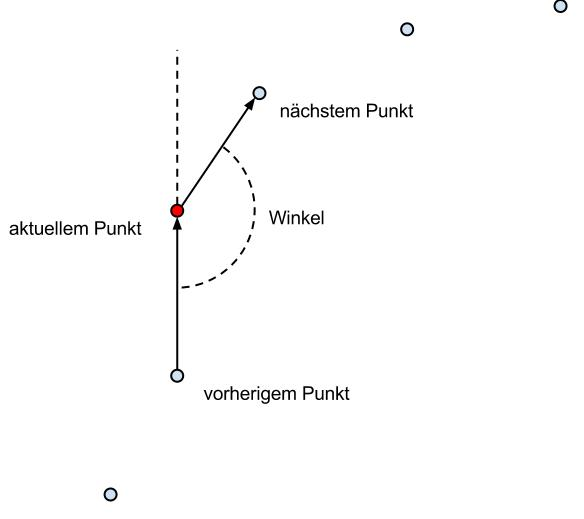
\includegraphics[width=0.5\textwidth]{feature_vektoren}
\caption{Vektoren}
\label{fig:feature_vektoren}
\end{center}
\end{figure}

Feature-Raum\\
Auswahl der für Training relevanten Features via Werkzeug\\
Aufteilung in Untermengen für Training, Test, Evaluation,...\\
Online-Bereitstellung der Features im Framework\\
% section Berechnung_der_benutzten_Features (end)


\section{Vergleiche, Korrelation} % (fold)
\label{sec:Vergleiche_Korrelation}
Ohne Korrelation. See figure ~\ref{fig:with-no-correlation}.\\

\begin{figure}[htbp]
\begin{center}
\subfigure{\label{fig:feature_with-no-correlation-gas}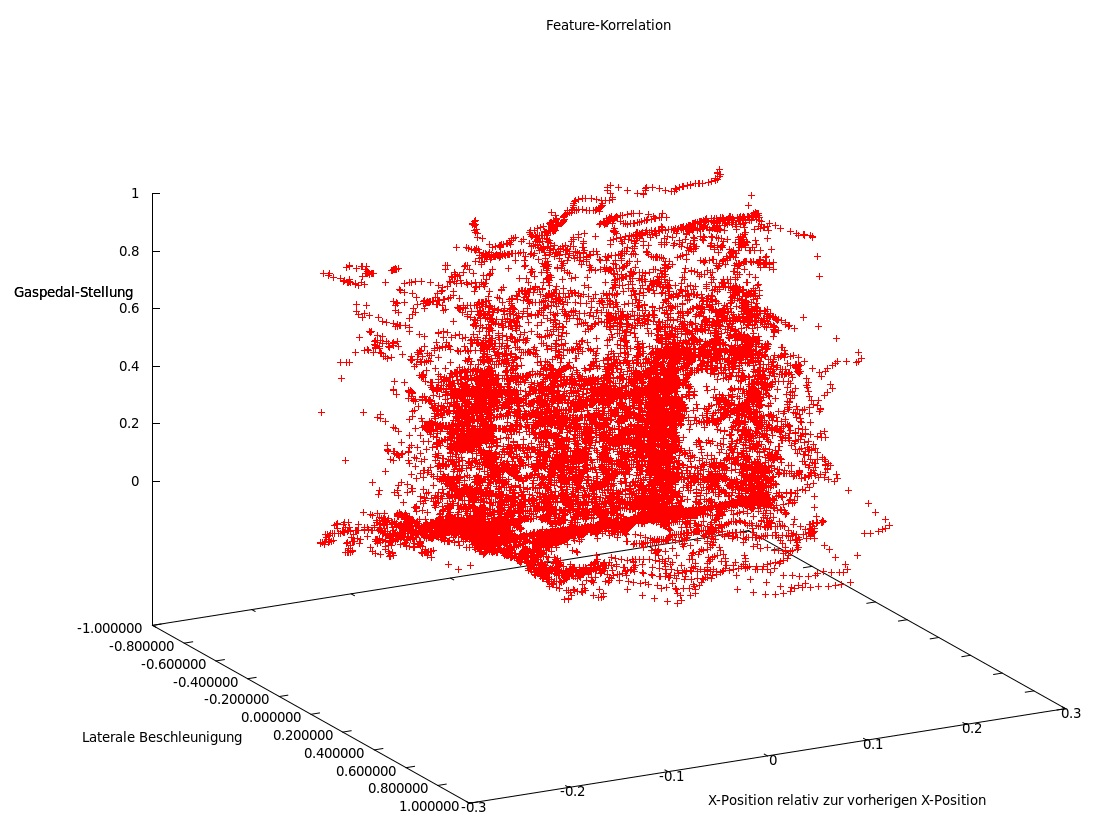
\includegraphics[width=0.45\textwidth]{feature_with-no-correlation-gas}}    
\hspace{1cm}            
\subfigure{\label{fig:feature_with-no-correlation-winkel}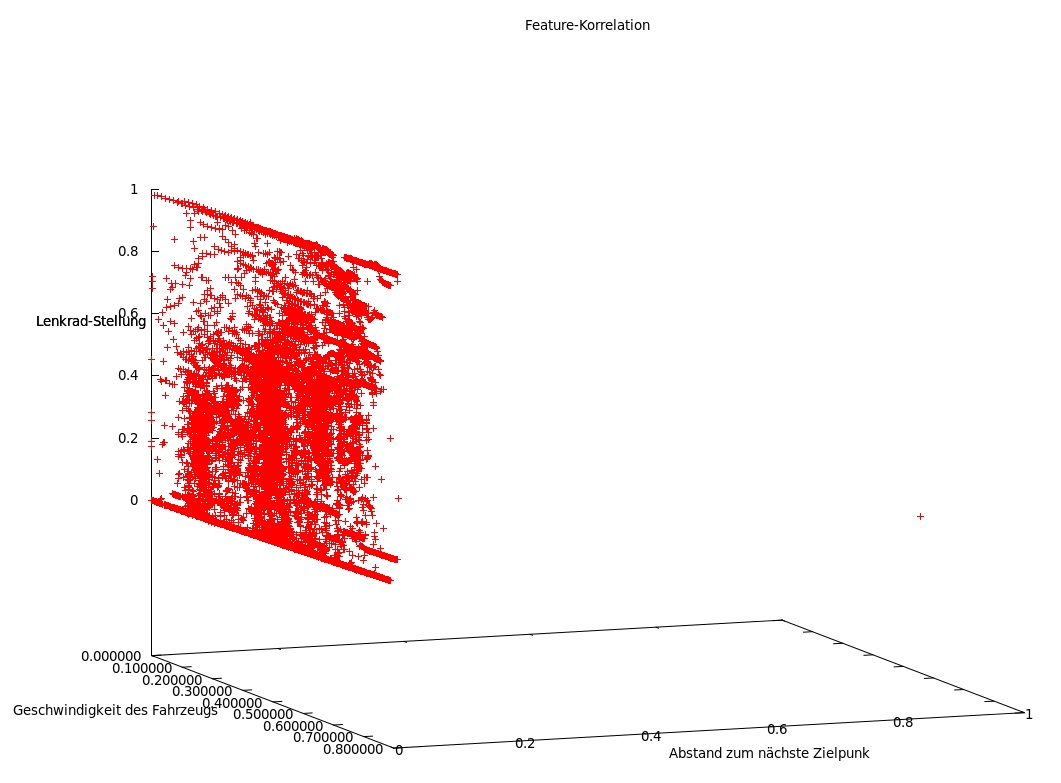
\includegraphics[width=0.45\textwidth]{feature_with-no-correlation-winkel}}
\caption{(a) No correlation gas. (b) no correlation winkel.}
\label{fig:with-no-correlation}
\end{center}
\end{figure}

Mit Korrelation. See figure ~\ref{fig:feature_with-correlation-gas}.\\

\begin{figure}[htbp]
\begin{center}
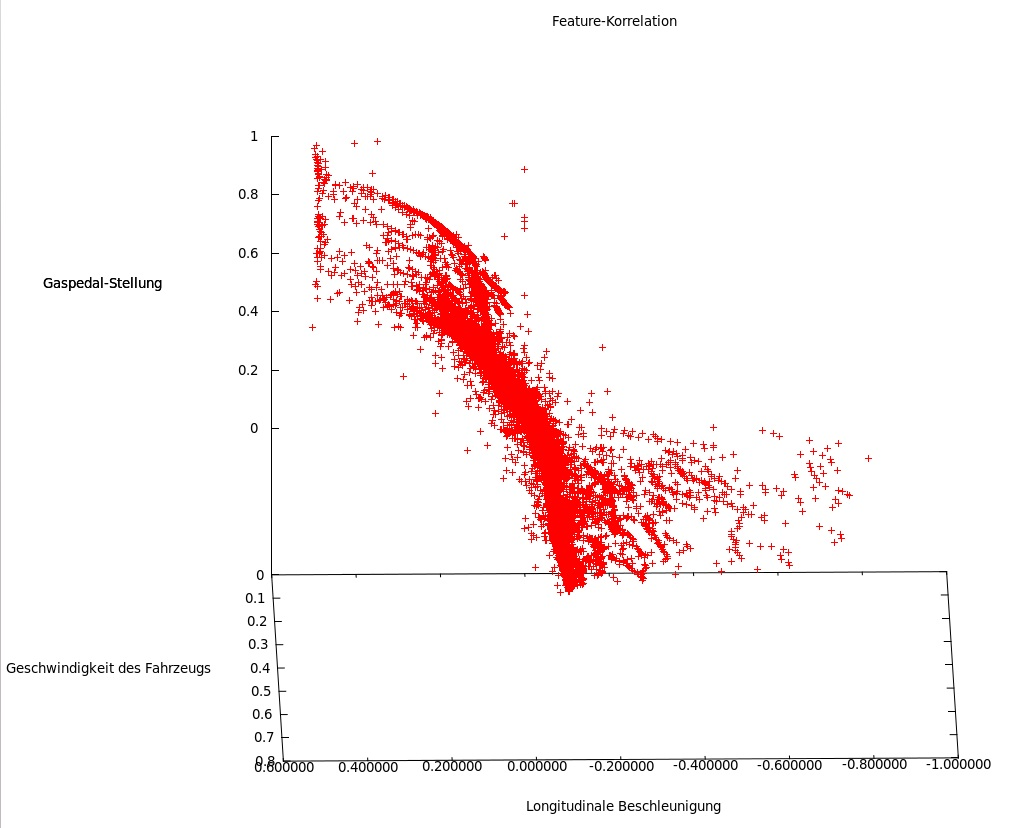
\includegraphics[width=0.5\textwidth]{feature_with-correlation-gas}
\caption{with-correlation-gas}
\label{fig:feature_with-correlation-gas}
\end{center}
\end{figure}

\begin{figure}[htbp]
\begin{center}
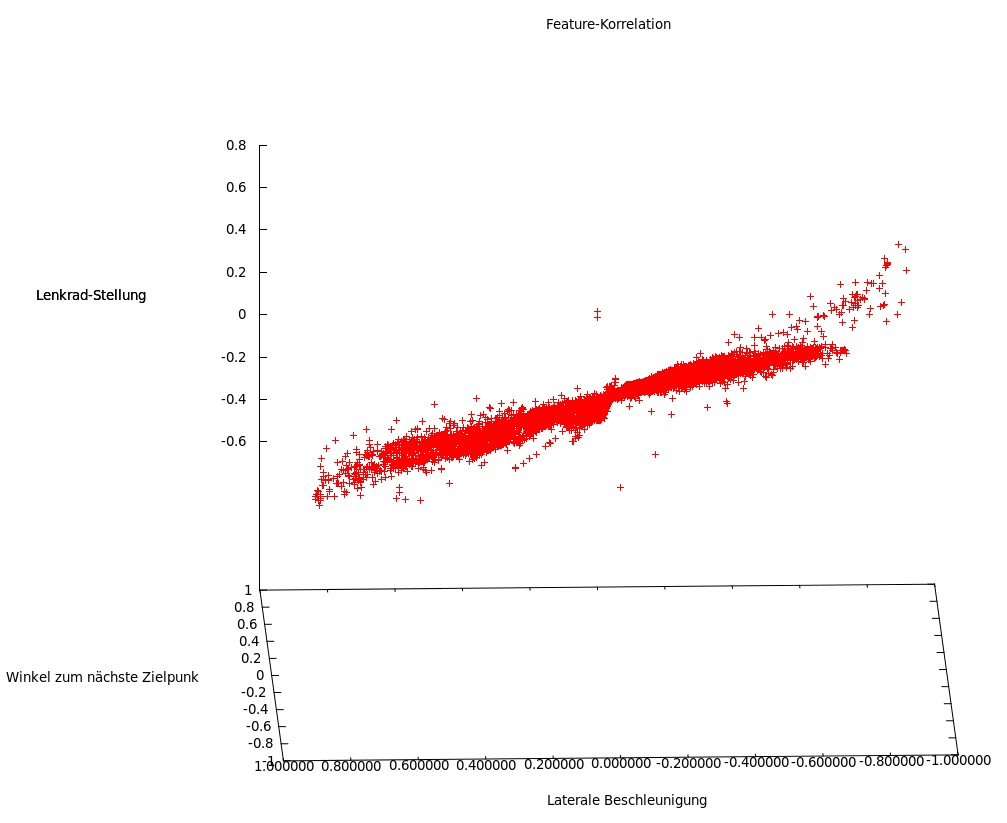
\includegraphics[width=0.5\textwidth]{feature_with-correlation-winkel}
\caption{with-correlation-winkel}
\label{fig:feature_with-correlation-winkel}
\end{center}
\end{figure}
% section Vergleiche_Korrelation (end)


\section{Verwendete Features} % (fold)
\label{sec:Berechnung_der_benutzten_Features}
6:  Laterale Beschleunigung\\
7:  Longitudinale Beschleunigung\\
9:  Geschwindigkeit des Fahrzeugs\\
18: Distanz vom Fahrzeug zum nächsten Punkt\\
19: Winkel vom Fahrzeug zum nächsten Punkt\\
...\\
Gas\\
Bremse\\
Winkel des Lenkrads\\
% section Verwendete Features (end)

% chapter Features (end)
